\chapter{Simulation Model Implementation}

\addcontentsline{toc}{chapter}{Simulation Model Implementation}

\section{Main Entities}

This chapter is going to describe the process of implementation, i.e. transition from a mathematical model to computer simulation. First of all we are going to create the basic elements that are essential to our model.

%\begin{figure}[!ht]
%  \centering
%  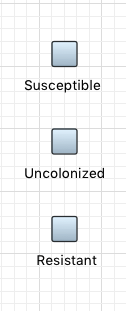
\includegraphics[height=0.5\textwidth]{img/screens/basic/basic4}
%  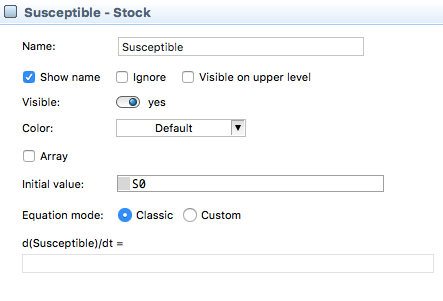
\includegraphics[height=0.5\textwidth]{img/screens/basic/basic3}
%  \caption{A picture of a gull.}
%\end{figure}

AnyLogic is a system that provides many useful components that can be used for modeling. The list of the available elements can be seen in the figure.

\begin{figure}[!ht]
  \centering
  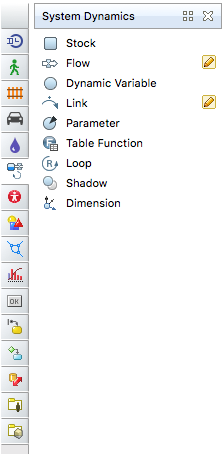
\includegraphics[height=0.5\textwidth]{img/screens/basic/basic22}
  \caption{The list of interactive elements used for System Dynamics models}
\end{figure}

\begin{figure}[!ht]
    \centering
    \begin{subfigure}[b]{0.3\textwidth}
        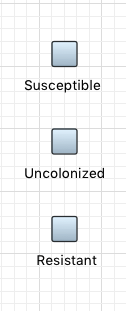
\includegraphics[width=0.5\textwidth]{img/screens/basic/basic4}
        \caption{The stocks of 3 observed groups}
    \end{subfigure}
    ~ %add desired spacing between images, e. g. ~, \quad, \qquad, \hfill etc.
      %(or a blank line to force the subfigure onto a new line)
    \begin{subfigure}[b]{0.6\textwidth}
        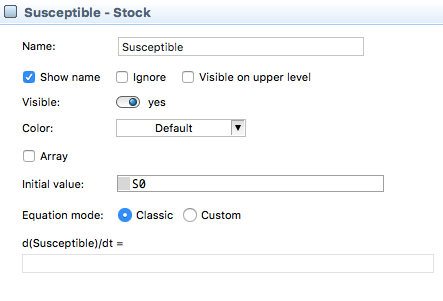
\includegraphics[width=\textwidth]{img/screens/basic/basic3}
        \caption{The properties of the Susceptible stock}
    \end{subfigure}
    \caption{Creation of the basic stock elements}
\end{figure}

Here we can see how every entity is treated in AnyLogic. There have been created three stocks for three different groups of the hospital population. We name every stock as Susceptible, Uncolonized and Resistant. Each stock needs to have an initial value, which indicates how many individuals were present in each group at the beginning. We call these initial values S0, X0 and R0 respectively.

\begin{figure}[!ht]
    \centering
    \begin{subfigure}[b]{0.48\textwidth}
        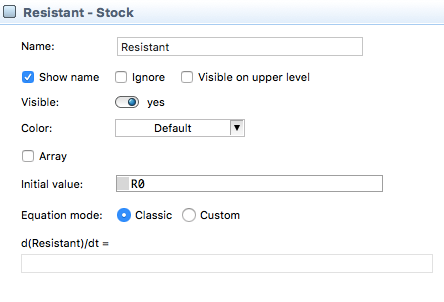
\includegraphics[width=\textwidth]{img/screens/basic/basic1}
        \caption{The properties of the Resistant stock}
    \end{subfigure}
    ~ %add desired spacing between images, e. g. ~, \quad, \qquad, \hfill etc.
      %(or a blank line to force the subfigure onto a new line)
    \begin{subfigure}[b]{0.48\textwidth}
        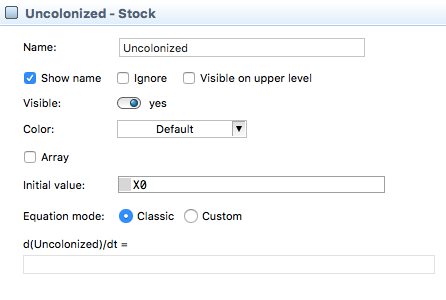
\includegraphics[width=\textwidth]{img/screens/basic/basic2}
        \caption{The properties of the Uncolonized stock}
    \end{subfigure}
    \caption{Properties of the basic stock elements}
\end{figure}

In order to set the initial values to the stocks, we will need to create so-called parameters, which are bound to the created stocks. Each parameter holds a value that will be set to the corresponding stock. After the start of model execution, the value of the actual stock may change, independent of the parameter. We create a parameter called S0 and connect it with the existing Susceptible stock.

\begin{figure}[!ht]
  \centering
  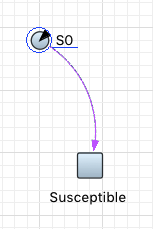
\includegraphics[height=0.5\textwidth]{img/screens/basic/basic8}
  \caption{Binding a parameter to Susceptible stock}
\end{figure}

When the Susceptible stock is connected with the created parameter, we can refer to that parameter when specifying the initial value of it. Since the stocks that we have created represent the probabilities of any individual to fall into one of the categories (susceptible, resistant or uncolonized), they should sum up to 1. Since we want to set approximately equal initial values to all three groups of people, we set S0 to be 0.33.

\begin{figure}[!ht]
  \centering
  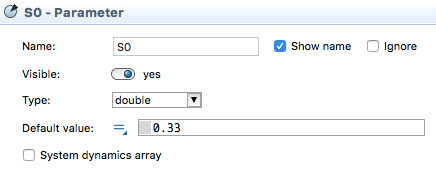
\includegraphics[width=0.5\textwidth]{img/screens/basic/basic7}
  \caption{Binding a parameter to Susceptible stock}
\end{figure}

After having connected the Susceptible stock with its parameter, we can do the same thing to Uncolonized stock. The parameter for its initial value will be called X0. The connection between the parameter and its stock is similar to the previous example.

\begin{figure}[!ht]
  \centering
  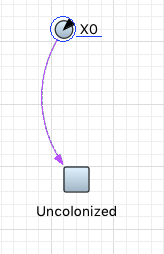
\includegraphics[height=0.5\textwidth]{img/screens/basic/basic9}
  \caption{Binding a parameter to Susceptible stock}
\end{figure}

The value of X0 will be the same that we have set to S0. On the following figure we can see how it is set to 0.33.

\begin{figure}[!ht]
  \centering
  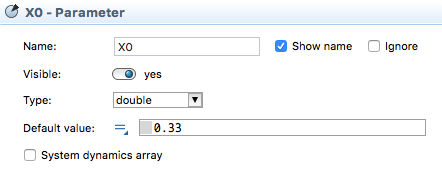
\includegraphics[width=0.5\textwidth]{img/screens/basic/basic6}
  \caption{Binding a parameter to Susceptible stock}
\end{figure}



% That's why we will set the initial values as 0.33, 0.33 and 0.34 (approximately equal values).

%\begin{figure}[!ht]
%    \centering
%    \begin{subfigure}[b]{0.48\textwidth}
%        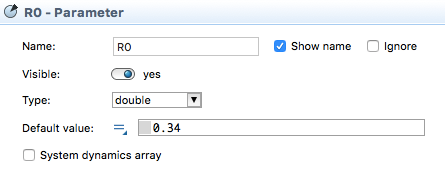
\includegraphics[width=\textwidth]{img/screens/basic/basic5}
%        \caption{The initial parameter for Resistant stock}
%    \end{subfigure}
%    ~ %add desired spacing between images, e. g. ~, \quad, \qquad, \hfill etc.
%      %(or a blank line to force the subfigure onto a new line)
%    \begin{subfigure}[b]{0.48\textwidth}
%        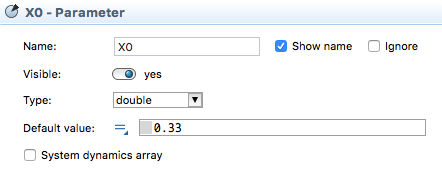
\includegraphics[width=\textwidth]{img/screens/basic/basic6}
%        \caption{The initial parameter for Uncolonized stock}
%    \end{subfigure}
%    ~ %add desired spacing between images, e. g. ~, \quad, \qquad, \hfill etc.
%      %(or a blank line to force the subfigure onto a new line)
%    \begin{subfigure}[b]{0.48\textwidth}
%        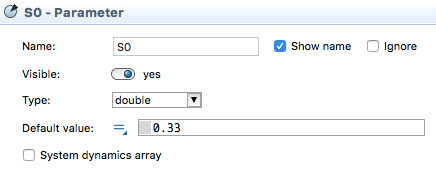
\includegraphics[width=\textwidth]{img/screens/basic/basic7}
%        \caption{The initial parameter for Susceptible stock}
%    \end{subfigure}
%    \caption{Parameters bound to the S, X, R stocks}
%\end{figure}